%-------------------------
% License : MIT
% Based on https://github.com/sb2nov/resume
% from Sourabh Bajaj
%------------------------
\documentclass[letterpaper,11pt]{article}

\usepackage{latexsym}
\usepackage[empty]{fullpage}
\usepackage{titlesec}
\usepackage{marvosym}
\usepackage[usenames,dvipsnames]{color}
\usepackage{verbatim}
\usepackage{enumitem}
\usepackage[pdftex]{hyperref}
\usepackage{fancyhdr}
\usepackage{graphicx}
%\usepackage{wrapfig}
\graphicspath{ {../images} }


\pagestyle{fancy}
\fancyhf{} % clear all header and footer fields
\fancyfoot{}
\renewcommand{\headrulewidth}{0pt}
\renewcommand{\footrulewidth}{0pt}

% Adjust margins
\addtolength{\oddsidemargin}{-0.375in}
\addtolength{\evensidemargin}{-0.375in}
\addtolength{\textwidth}{1in}
\addtolength{\topmargin}{-.5in}
\addtolength{\textheight}{1.0in}

\urlstyle{same}

\raggedbottom
\raggedright
\setlength{\tabcolsep}{0in}

% Sections formatting
\titleformat{\section}{
  \vspace{-4pt}\scshape\raggedright\large
}{}{0em}{}[\color{black}\titlerule \vspace{-5pt}]

%-------------------------
% Custom commands
\newcommand{\resumeItem}[2]{
  \item\small{
    \textbf{#1}{: #2 \vspace{-2pt}}
  }
}

\newcommand{\resumeSubheadingShort}[4]{
  \vspace{-1pt}\item
    \begin{tabular*}{12.5cm}{l@{\extracolsep{\fill}}r}
      \textbf{#1} & #2 \\
      \textit{\small#3} & \textit{\small #4} \\
    \end{tabular*}\vspace{-5pt}
}

\newcommand{\resumeSubheading}[4]{
  \vspace{-1pt}\item
    \begin{tabular*}{0.97\textwidth}{l@{\extracolsep{\fill}}r}
      \textbf{#1} & #2 \\
      \textit{\small#3} & \textit{\small #4} \\
    \end{tabular*}\vspace{-5pt}
}

\newcommand{\resumeSubItem}[2]{\resumeItem{#1}{#2}\vspace{-4pt}}

\renewcommand{\labelitemii}{$\circ$}

\newcommand{\resumeSubHeadingListStart}{\begin{itemize}[leftmargin=*]}
\newcommand{\resumeSubHeadingListEnd}{\end{itemize}}
\newcommand{\resumeItemListStart}{\begin{itemize}}
\newcommand{\resumeItemListEnd}{\end{itemize}\vspace{-5pt}}

%-------------------------------------------
%%%%%%  CV STARTS HERE  %%%%%%%%%%%%%%%%%%%%%%%%%%%%


\begin{document}

\begin{tabular*}{\textwidth}{l@{\extracolsep{\fill}}r}
  \textbf{\Large Joshua Martínez} & Email : \href{mailto:djoshuamartinezpineda@gmail.com}{djoshuamartinezpineda@gmail.com}\\
  \href{https://mynjj.github.io}{https://mynjj.github.io} &  \\
\end{tabular*}

%\vspace{55pt}
\begin{tabular*}{\textwidth}{l@{\extracolsep{\fill}}r}
  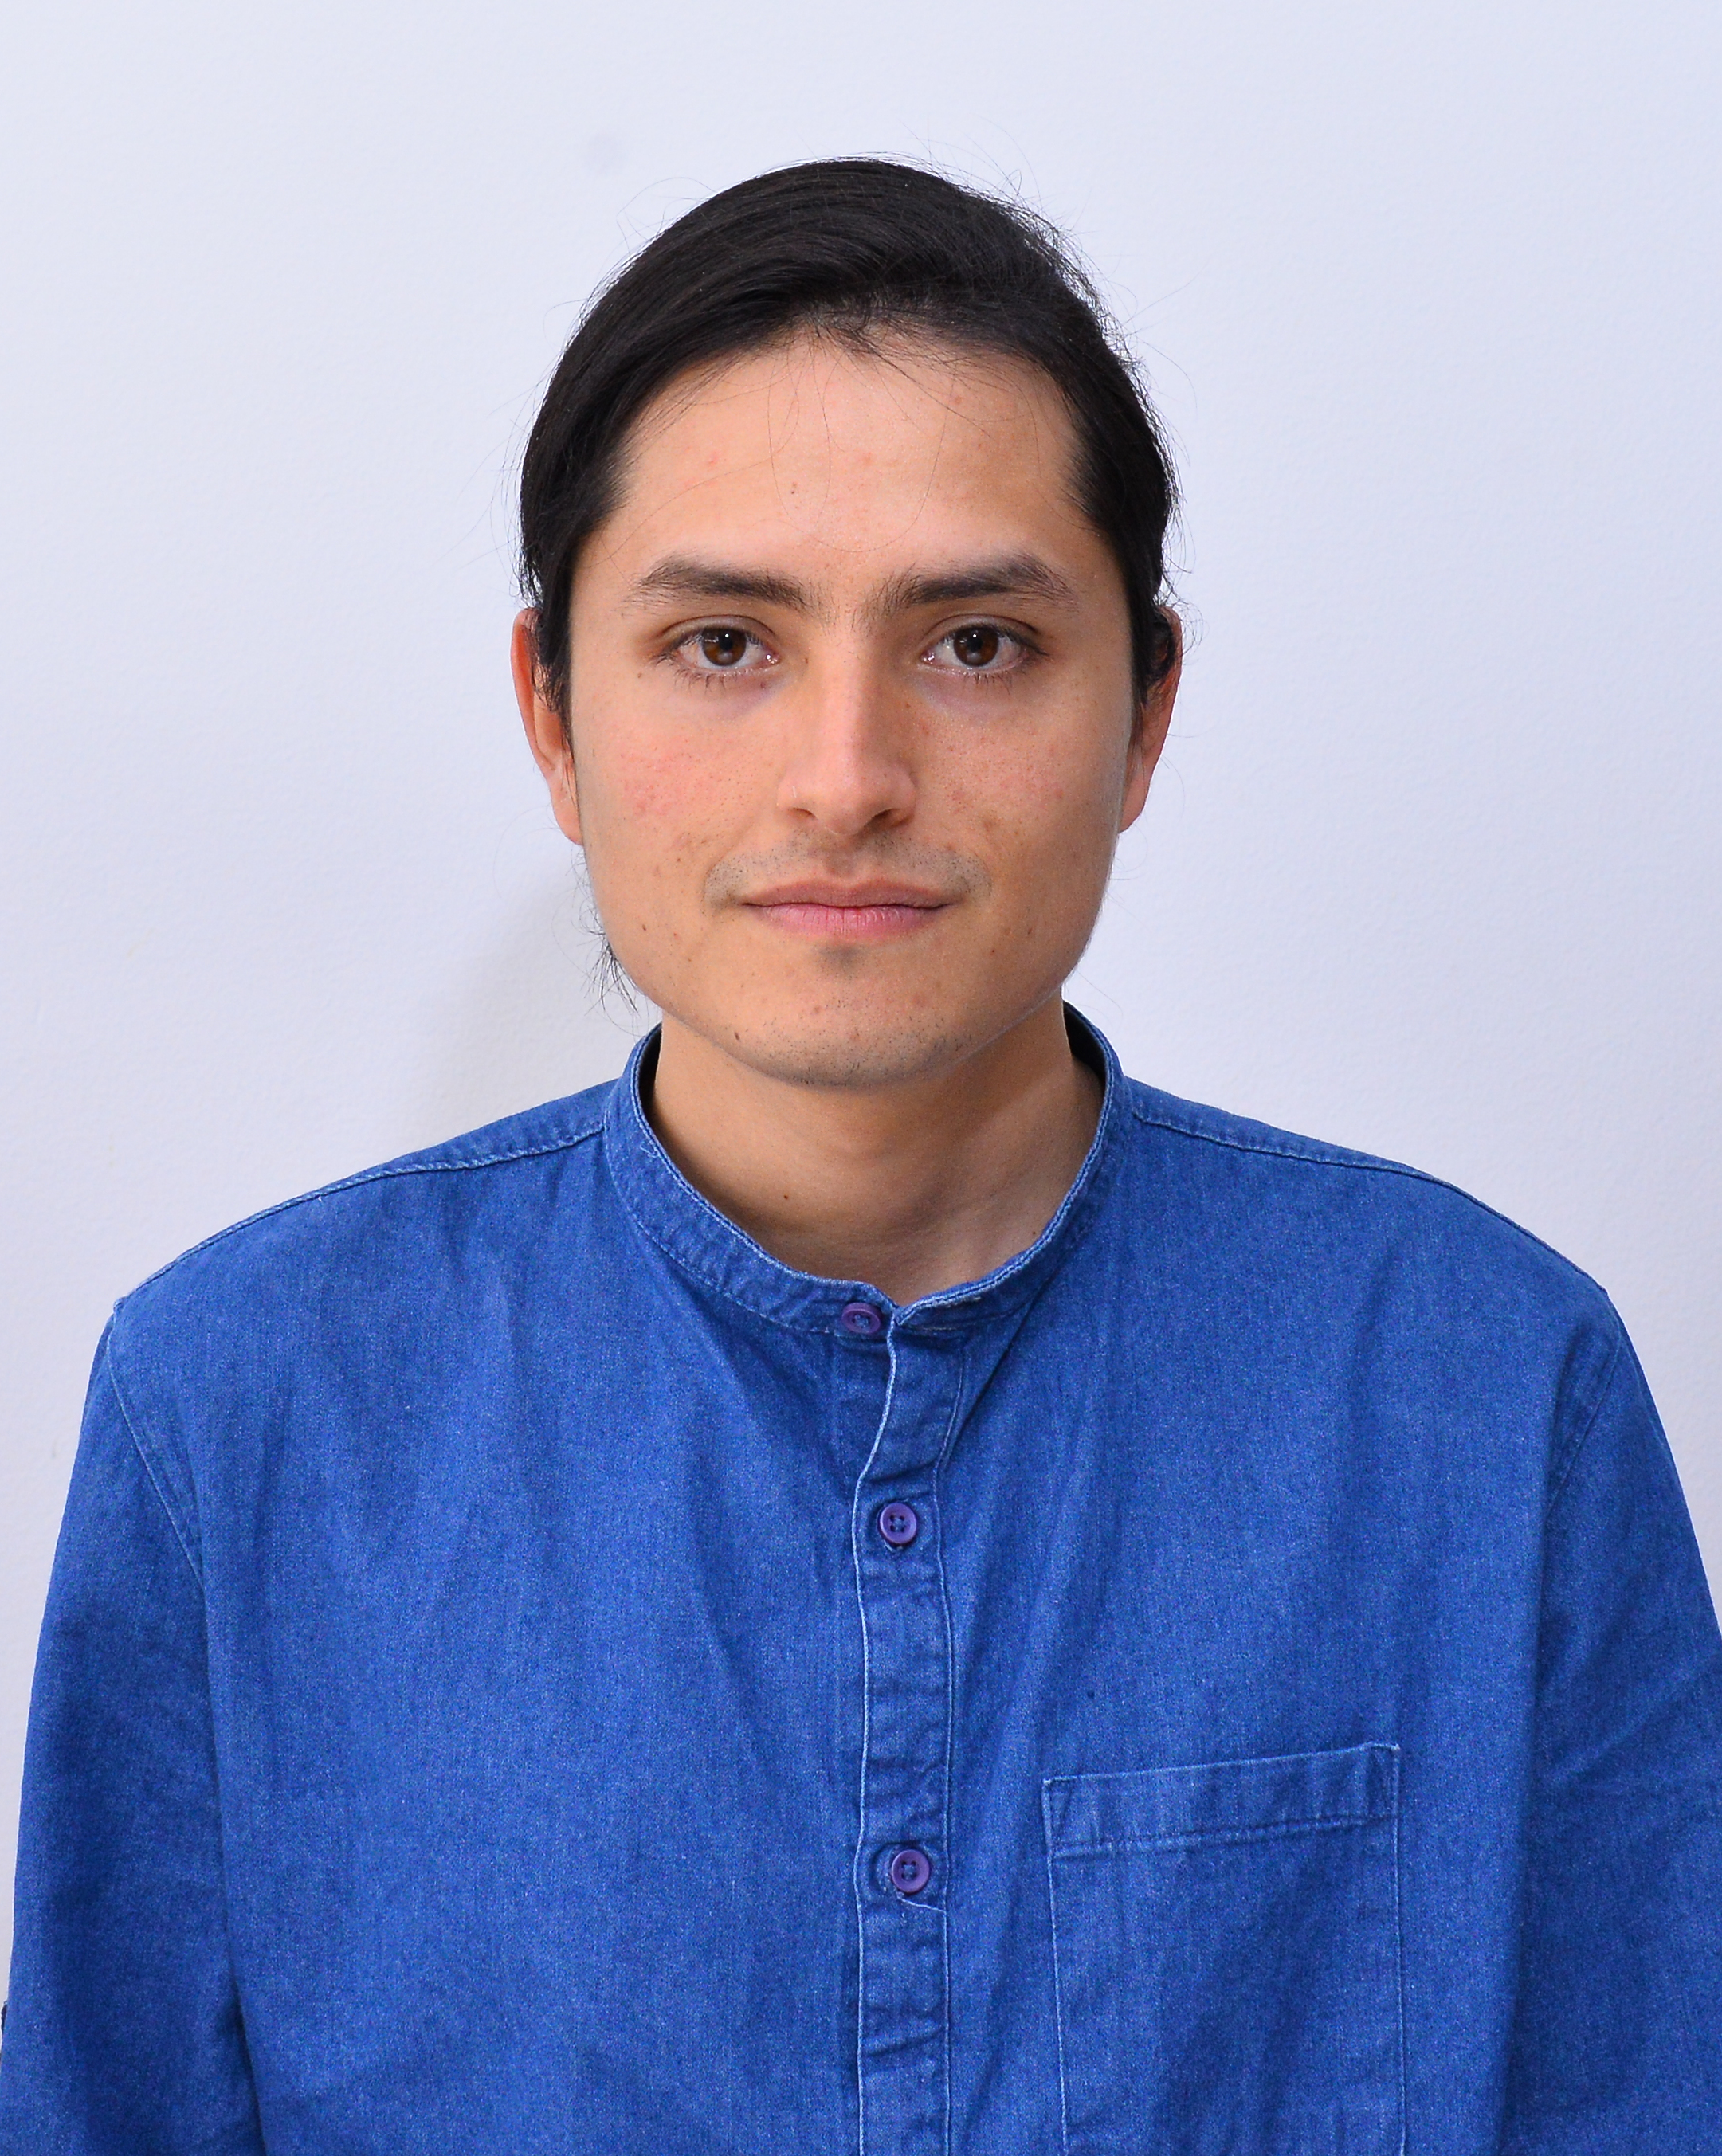
\includegraphics[width=5cm, keepaspectratio]{formal_me.JPG} & 
  \parbox[b]{13cm}{
    \section{Profile}
  Hardworking passionate profesional, currently studying a \textbf{Msc. in Computer Science}. With 
  experience in software development. Highly responsible on my work. Excited to learn more, try new
things, face challenges, and to help.
\section{Education}
  \resumeSubHeadingListStart
    \resumeSubheadingShort
      {IT University}{Copenhaguen, Denmark}
      {\parbox{6.5cm}{Master of Science in Computer Science}}{Aug. 2020 -- Present}
    \resumeSubheadingShort
      {Universidad La Salle}{Mexico City, Mexico}
      {\parbox{6.5cm}{Bachelor of Engineering in Electronics and Communications}}{Aug. 2012 -- Nov. 2016}
  \resumeSubHeadingListEnd
  }

\\
\end{tabular*}
  \resumeSubHeadingListStart
    \resumeSubheading
      {Universidad Nacional Autónoma de México}{Mexico City, Mexico}
      {Bachelor of Mathematics}{Aug. 2014 -- Jul. 2018}
  \resumeSubHeadingListEnd

\section{Experience}
  \resumeSubHeadingListStart


  \resumeSubheading
      {Microsoft}{Copenhagen, Denmark}
      {Student Worker}{Sept. 2021 - Present}

  \resumeSubheading
      {Microsoft}{Copenhagen, Denmark}
      {Engineering Intern}{Jul. 2021 - Aug. 2021}

  \resumeSubheading
      {DFDS}{Copenhagen, Denmark}
      {Student Developer}{Apr. 2021 - Jun. 2021}

      Mainly work on \textbf{TS/React}, maintenance of shared components library. I learned a lot from the project structure and the tools used by the team.
  
  \resumeSubheading
      {ABaCus DK}{Copenhagen, Denmark}
      {Student Developer}{Nov. 2020 - May 2021}

    Wrote fixes for bugs. Also the frontend and backend for pages
        displaying statistics for the teacher and students. The project used
        \textbf{PHP/Symfony}, \textbf{JS/React}.

    \resumeSubheading
      {TIDE}{Mexico City, Mexico}
      {Software Engineer}{Jan. 2019 - Aug. 2020}
      \vspace{3pt}

      I developed many useful skills, learned to deliver fully functional
      products and to take responsability for them as a team. Designed and implemented
      creative solutions with several technologies.
      \resumeItemListStart
        \resumeItem{Employee time clock}
          {\textbf{Raspberry Pi's} with multiple identification and synchronization features. Integrated
            \textbf{sensors SDK's} (\textbf{C/Java}), implemented features for the main service
            (\textbf{Node.js}), and UI(\textbf{React})}
        \resumeItem{Airport Lounge app}
          {Android/iOS app with \textbf{React Native}. Several features, integrated to an
          existing backend and created a backend-for-frontend for other features
          (\textbf{Node.js/sails.js}). Other technologies used: \textbf{Redux}, \textbf{Firebase FCM}}
        \resumeItem{Scotiabank's online pride parade}
        {Basic MMORPG for 2020's stay@home Pride Parade. \textbf{AWS/EC2} instances
          running a \textbf{Phaser.js} game, connecting to \textbf{WebSocket} servers (\textbf{Typescript}). \textbf{Redis} 
          used for chat features.}
        \resumeItem{IOT devices monitor}
          {Utilities to provide software updates, remote \textbf{SSH} access and stats
            recopilation for remote technical support. Implemented features on
            both sides (\textbf{Node.js}, \textbf{PHP/Symfony}, \textbf{React}, \textbf{Linux scripting}).}
        \resumeItem{Coca-cola promotional game}
          {Soccer game for marketing stands of Coca-cola running on \textbf{Raspberry Pi's},
            controlled by a Wii controller. Created with \textbf{Python/Pygame}.}
        \resumeItem{Airport Lounge software}
          {Software spanning several company areas. Implemented several
            features, on both backend (\textbf{PHP/Symfony}) and frontend (\textbf{React/Redux}).}
        \resumeItem{Restaurant software}
          {Highly customized restaurant software. Implemented several features,
            on both backend (\textbf{PHP/Symfony}) and frontend (\textbf{React/Redux}).}
      \resumeItemListEnd

    \resumeSubheading
      {VtSoftware}{Playa del Carmen, Mexico}
      {Software Engineer}{Jun. 2017 - May 2018}
      \vspace{3pt}

      I learned how to translate my academic knowledge to useful software. One
      of the most important skills I learned is to listen to the client
      requirements and design accordingly.

      \resumeItemListStart
        \resumeItem{Vacation Clubs Payroll Software}
          {Modeled and designed according to customer needs. Bootstraped
            project on \textbf{PHP/Laravel} and \textbf{Vue.js}, integrated to an existing sales
            system DB. Also wrote some \textbf{SQLServer} stored procedures.}
        \resumeItem{Hotel Inventory Software}
          {Modeled and designed according to customer needs. Bootstraped project
          on \textbf{PHP/Laravel} and \textbf{jQuery}.}
      \resumeItemListEnd

    \resumeSubheading
      {École de Technologie Supérieure}{Montreal, Canada}
      {Research Internship}{Apr. 2015 - Jul. 2015}
      \resumeItemListStart
        \resumeItem{Estimation of disparity on GPUs}
          {Research on disparity estimation algorithms and implementation on
            \textbf{Matlab} and then using \textbf{C/CUDA}}
      \resumeItemListEnd

  \resumeSubHeadingListEnd

\section{Other experience}
\resumeSubHeadingListStart
\resumeSubItem{Teaching activities}{Private tutor on mathematics and
  programming, mostly focusing on kids (from 9 to 16). Social Service as an
  English teacher for adults.}
\resumeSubHeadingListEnd


\section{Academic activities}
  \resumeSubHeadingListStart
    \resumeSubItem{ANFEI's award}{Highest GPA on engineering faculty. Graduated with
      Magna Cum Laude.}
    \resumeSubItem{Robotics Winter School. 2013}{INAOE, Puebla, Mexico.}
    \resumeSubItem{Robotics competitions. 2011 - 2013}
      {Participation on Robocup, LARC competitions with the school robotics team
        (Cyberlords). Istanbul, Turkey and Mexico City.}
    \resumeSubItem{Programming competitions.}
      {IEEExtreme Programming competitions.}
  \resumeSubHeadingListEnd

  \section{Skills I've worked with}
  \vspace{-30pt}
\begin{tabular}{p{9cm}p{9cm}}
  \section{Programming Languages}
  JS, TS, Node.js, Python, C, Java, SQL, PHP, Matlab
  \hfill &

  \section{Technologies}
    \resumeItemListStart
    \resumeSubItem{Frontend}{React, Redux, React Native, Vue.js, Phaser, eCharts.}
    \resumeSubItem{Backend}{Laravel, Symfony, Redis, Socket.io, Express, Sails.js}
    \resumeSubItem{Other}{Linux, Raspberry Pi, AWS, Git, SVN, Nginx, Matlab}
    \resumeItemListEnd
  \end{tabular}

  \section{Other skills (Coursework \& others)}
    Scala, C++, Microchip PIC Assembler, Arduino, Eagle, \LaTeX.

  \section{Languages}
  \resumeItemListStart
  \resumeSubItem{Spanish}{Native}
  \resumeSubItem{English}{Fluent. TOEFL iBT(115/120)}
  \resumeItemListEnd


\end{document}
